\documentclass[12pt]{article}
\usepackage[utf8]{inputenc}
\usepackage{graphicx} 
\usepackage{fancyhdr} 
\usepackage{geometry} 
\usepackage{hyperref}
\hypersetup{colorlinks=true}
\linespread{1} 
\setlength{\parindent}{0pt} 
\setlength{\parskip}{1em} 
\usepackage[format=plain,
            font=it]{caption} 
\usepackage[english]{babel}
\usepackage{csquotes}
\renewcommand{\headrulewidth}{0pt}
\geometry{letterpaper, portrait, margin=1in}
\setlength{\headheight}{14.5pt}

\newcommand\titleofdoc{Comparison Based Implementation of a Single Instance of BlackJack} 

\begin{document}
\begin{titlepage}
   \begin{center}
        \vspace*{3cm} 
        \Huge\textbf{\titleofdoc : Project Report}
        
        \Large{Rangasri Chakravarthy , Priyanka Dutta}
        \Large{(rachakra@ucsc.edu, pdutta1@ucsc.edu)}
        
        \href{https://github.com/RangasriChakravarthy/BlackJack.git}{BlackJack : GitHub link}
       
    \end{center}
    
\section*{Abstract} 

In this project, we've explored implementing a simplified version of the well-known game of BlackJack in 4 different languages: C++, Scala, Java, Python. We've also developed elaborate test cases to validate different scenarios that might occur in a game of BlackJack, using Mock in Python, JUnit in Java and FreeSpec in Scala. We then compared the lines of code, challenges we faced, performance analysis of running the program via command line and running test cases for each of the 4 languages.
\end{titlepage}

\setcounter{page}{2}
\pagestyle{fancy}
\fancyhf{}
\rhead{\thepage}
\lhead{\titleofdoc}

 

\section{Introduction}
BlackJack is a card game. We've assumed that there will be a player (played by us through command line) and a dealer (played by the system). We've used a standard deck of 52-cards. This deck has:
\begin{itemize}
  \item 'number cards' with a face value of 2-10, worth the number on the card
  \item 'face cards' (King, Queen, Jack), each worth 10 points
  \item 'aces' (Ace), worth 1 or 11 points. We've discussed about this in Ace scoring section.
\end{itemize}

These are some of the definitions of terms we've used in the rest of this document:

\textbf{Hand}: a collection of cards that a player or dealer owns for the duration of the game.

\textbf{Hit}: add another card to the player/ dealer's hand

\textbf{Stand}: add no more cards; stop playing a turn; proceed to the next phase of the game.

\textbf{Bust}: more than 21 points in hand; the turn is instantly over and the player/ dealer has lost.

\subsection{Scoring}

Calculating the score is done by adding the points of all cards at hand. 

Say the player was dealt 6 and Q:

[6 \quad Q] \Rightarrow 6 + 10 = 16

At this point, if the player Hits and gets a 7,

[6 \quad Q \quad 7] \Rightarrow 6 + 10 + 7 = 23

23 is over 21 so they would have busted, and the game ends.

\textbf{Ace Scoring:} An ace can be worth one or eleven points. At any point in the game, there is a single "optimal" value for the ace card. Our program determines and reports that value. Here's an example to better understand this scenario. 

If the cards at Hand are 7 and A,

[7 \quad A] \Rightarrow 7 + 11 = 18

The optimal value for the ace is always the one that creates the greatest non-busted hand value. In this case, that is an 11. If a player decides to hit at this point, they will likely bust with the ace valued at 11. But, the value is re-assessed every time a card is dealt. 

Let's look at multiple aces in hand: with a starting hand of A A there are three possible hand values: 2 (1 + 1), 12 (11 + 1), or 22 (11 + 11) , which is a bust. What happens when another ace is added? Here's how our algorithm works:

[A \quad A \quad A] \Rightarrow 11 + 1 + 1 = 13

Note that any hand with more than one ace as an 11 will be a bust. So our algorithm handles this condition to avoid busting.

\subsection{Winning}

Each player's objective is to get as close to 21 points as possible without going over.
The player tries to outscore the dealer, despite not knowing the dealer's score.

The dealer plays by a simple rule: hit until the hand's score is greater than or equal to 17 ("stand on 17"). In our game there is no betting, no splitting, no doubling down.

\section{Implementation}

We implemented this project in an object oriented style in all 4 languages. We used 2 classes, Deck class and Game class in Python, Java and C++. In Scala, we used Object for Deck and Game.

Implementation of a deck of cards in Python: 
cards\_ordered = ['A', 'K', 'Q', 'J', '2', '3', '4', '5', '6', '7', '8', '9', '10'] * 4

Data structure we used to initialize the deck of cards in other languages:
\begin{itemize}
    \item Scala: ListBuffer[String]
    \item Java: List $\langle String \rangle$
    
    \item C++: vector $\langle string \rangle$
\end{itemize}

\textbf{Methods:} We have randomized the cards that will be dealt during play by using a \textbf{shuffle\_cards()} function and we used \textbf{random\_draw()} function which randomly picks one card from the shuffled deck of cards.

We've developed a method called \textbf{compute\_score()} that is called to calculate the score of a player or dealer's hand. This method also handles the ace scoring that we discussed previously.

All 52 cards are present in the deck at the start of the game. The game starts with dealing cards. The \textbf{deal\_initial\_dealer\_cards()} function is used to deal two cards to the dealer: one face up, one face down. The \textbf{deal\_initial\_player\_cards()}  function is used to deal two cards to the player: both face up.

The main part of the game is handled by two functions, namely: \textbf{player\_game()} and \textbf{dealer\_game()}. To run these functions, we've used 2 Boolean flags, \textbf{game\_over} (initialized as false) and \textbf{player\_input\_to\_continue}. The \textbf{player\_game()} asks the player whether they want to Hit or Stand. The flag \textbf{player\_input\_to\_continue} is set to true as long as the player keeps hitting and it is set to false when the player stands. The player can continue to hit as many times as they wish until they Stand or Bust. When the player chooses to stand, their turn is over; they have no further opportunity to get more cards. If at any point the player's score goes over 21, they have busted and lost the game. At this point, the game ends and the \textbf{game\_over} flag is set to true.

If at any point the player gets exactly 21, they instantly win and the game is over.The system points out that the player won with a blackjack!

Once the player Stands, and the \textbf{game\_over} flag is still false, the \textbf{dealer\_game()} is called to play the dealer's turn. The dealer's face down card (denoted by ?) is revealed. The dealer then plays by a simple set of rules: Hit until the hand's score is greater than or equal to 17. If at any time the dealer busts, the game is over; the player wins. Otherwise, at some point the dealer will stand. At that point, the program calculates the scores of dealer and player and whoever has the highest score wins the game. If both hands have the same score, the result is a tie. At this point the game ends.

\subsection{Test implementation}

We developed various test scenarios to validate our program:
\begin{itemize}
    \item \textbf{test\_score\_compute()} to check the compute\_score()
    \item \textbf{test\_deal\_cards()} to check if 2 cards are dealt to the dealer and player initially and that the dealt cards are removed from the deck.
    \item \textbf{test\_player\_blackjack()} to check when the player hits blackjack from initial serve (AK/ AQ/ AJ/ A10)
    \item \textbf{test\_player\_bust()} to check if the player busts (player\_score$>$21)
    \item  \textbf{test\_player\_tie()}to check when the player stands and dealer stands and its a tie (player\_score == dealer\_score)
    \item \textbf{test\_dealer\_bust()} to check when the player stands and dealer busts (dealer\_score$>$21)
    \item \textbf{test\_player\_stand\_win()} to check when the player stands and dealer stands and player wins ( player\_score $>$ dealer\_score)
    \item \textbf{test\_dealer\_stand\_win()} to check when the player stands and dealer stands and dealer wins ( player\_score $<$ dealer\_score)
    \item \textbf{test\_both\_blackjack()} to check when both dealer and player are dealt blackjack cards (AK/ AQ/ AJ/ A10), then, the player wins.
\end{itemize}

To develop these tests, we used the mock library in Python, FreeSpec from the scalatest library in Scala and JUnit tests for Java.

\begin{figure}[h] 
\centering
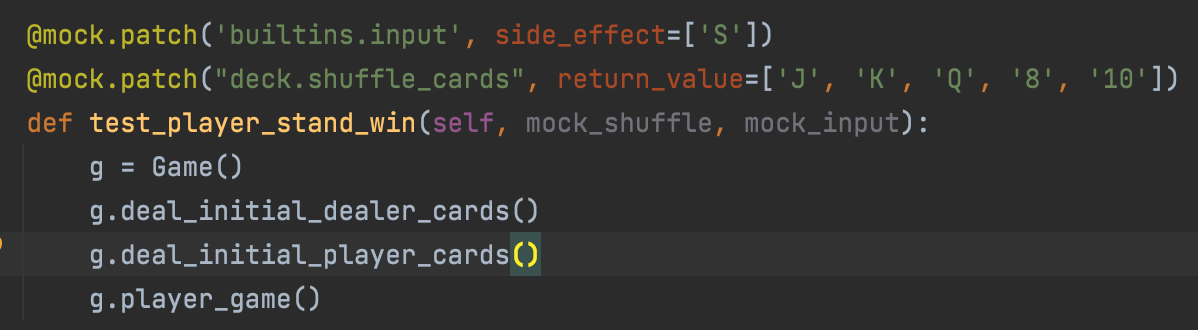
\includegraphics[height=6cm, width=15cm]{PythonMock.png}
\caption{An example mock test scenario in Python}
\end{figure}

\begin{figure}[h] 
\centering
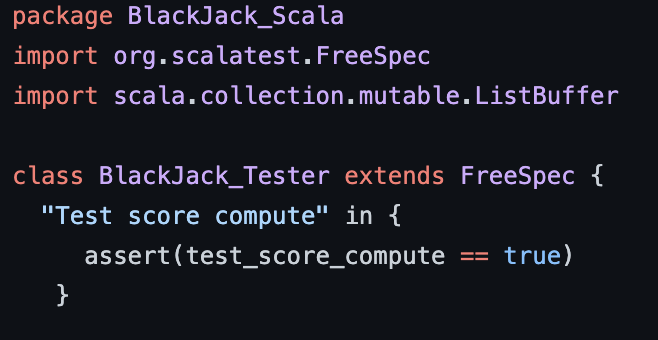
\includegraphics[height=6cm, width=15cm]{ScalaTest.png}
\caption{An example test scenario in Scala}
\end{figure}
\pagebreak

\begin{figure}[h] 
\centering
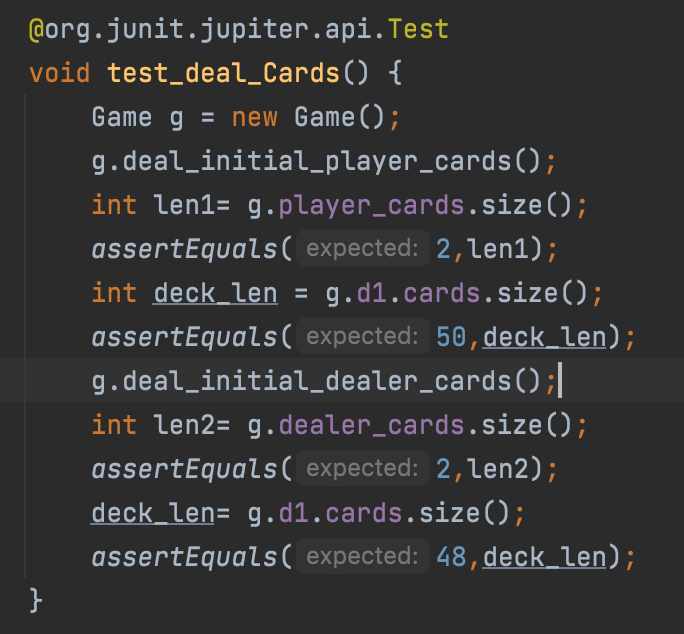
\includegraphics[height=8cm, width=10cm]{JavaTest.png}
\caption{An example JUnit test scenario in Java}
\end{figure}

\section{Results}

We defined a set of rules for the game implementation and we designed a program in all 4 languages as uniformly as possible. Here are screenshots of some scenarios we captured in 4 different languages. 

\begin{figure}[h!]
\centering
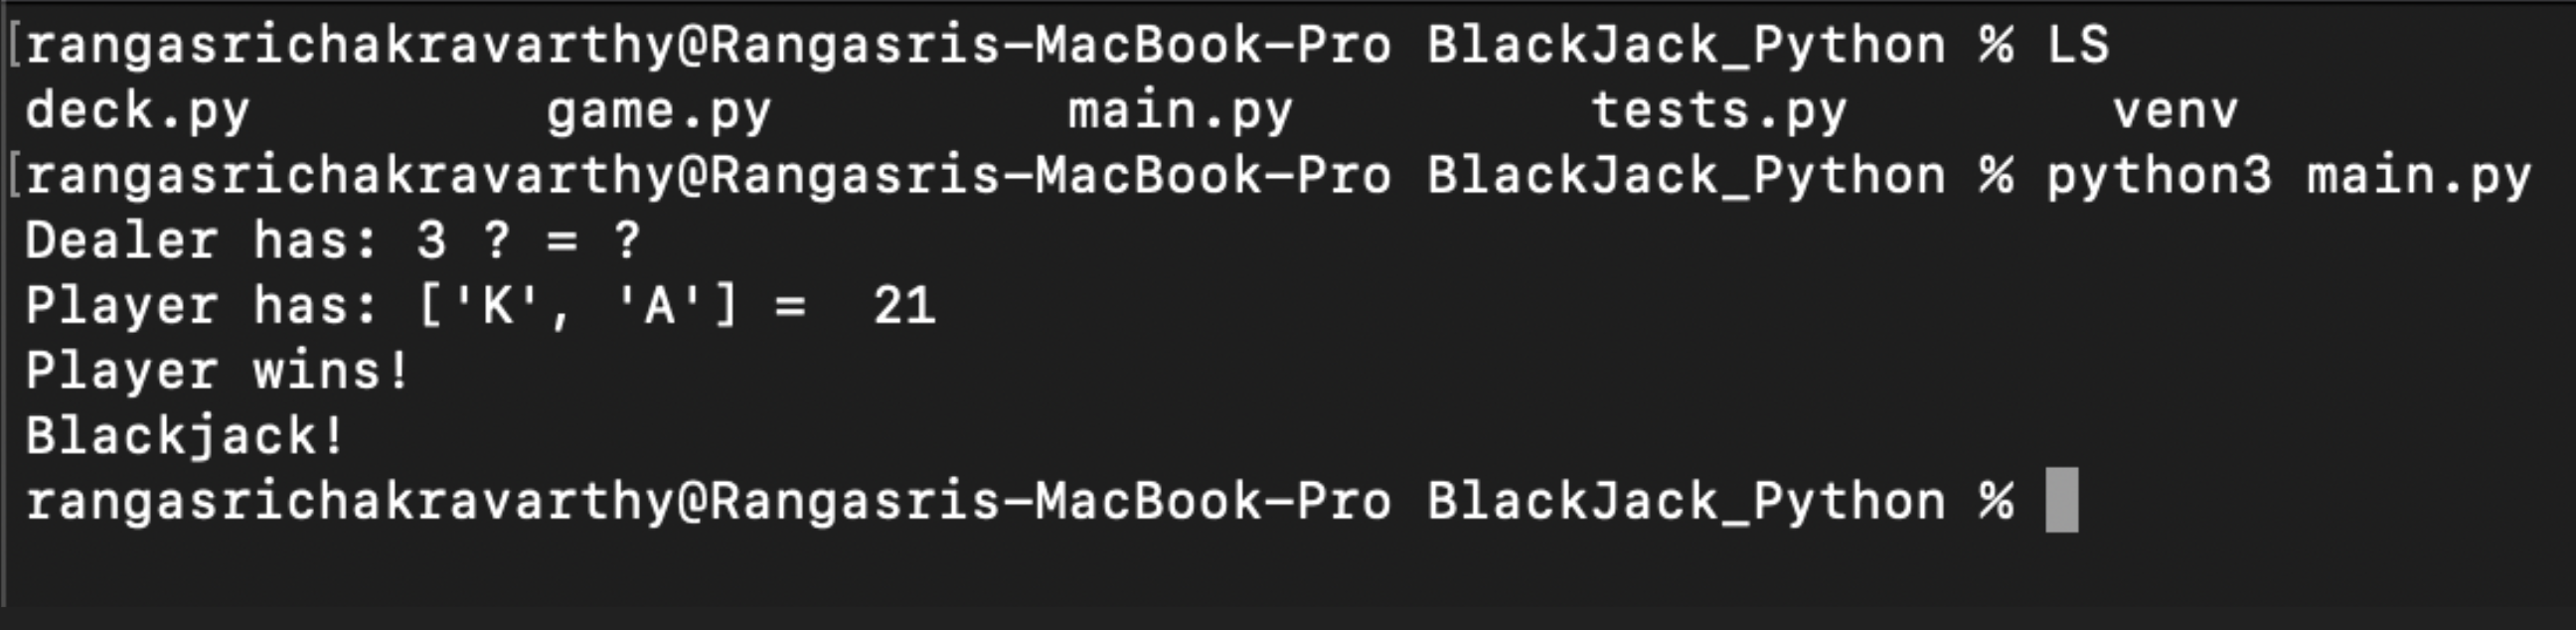
\includegraphics[height=6cm, width=15cm]{Python.png}
\caption{An example scenario of a player blackjack, that we've captured in Python}
\end{figure}

\pagebreak

\begin{figure}[ht!] 
\centering
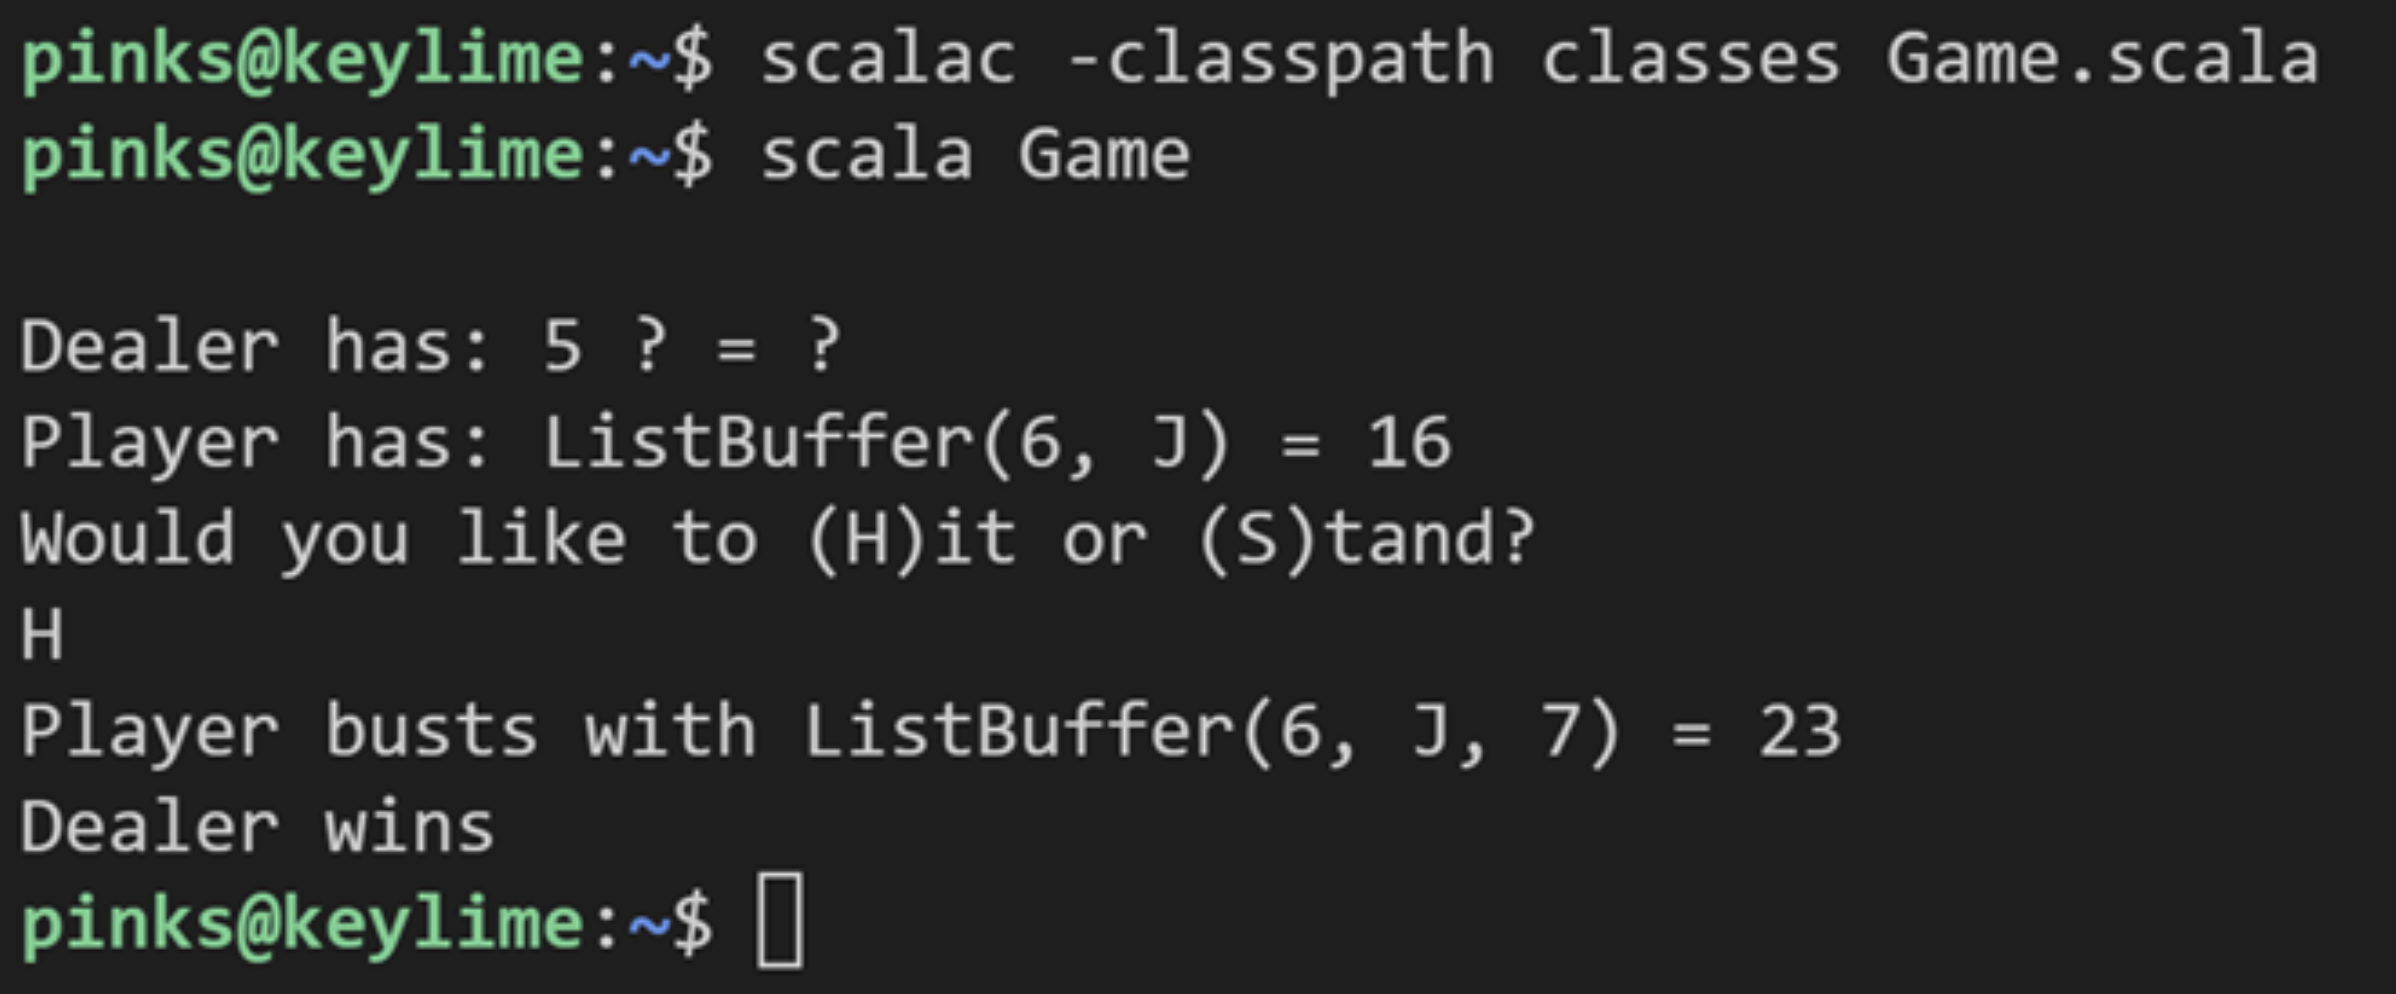
\includegraphics[height=5cm, width=15cm]{Scala.png}
\caption{An example scenario of a player busting, that we've captured in Scala}

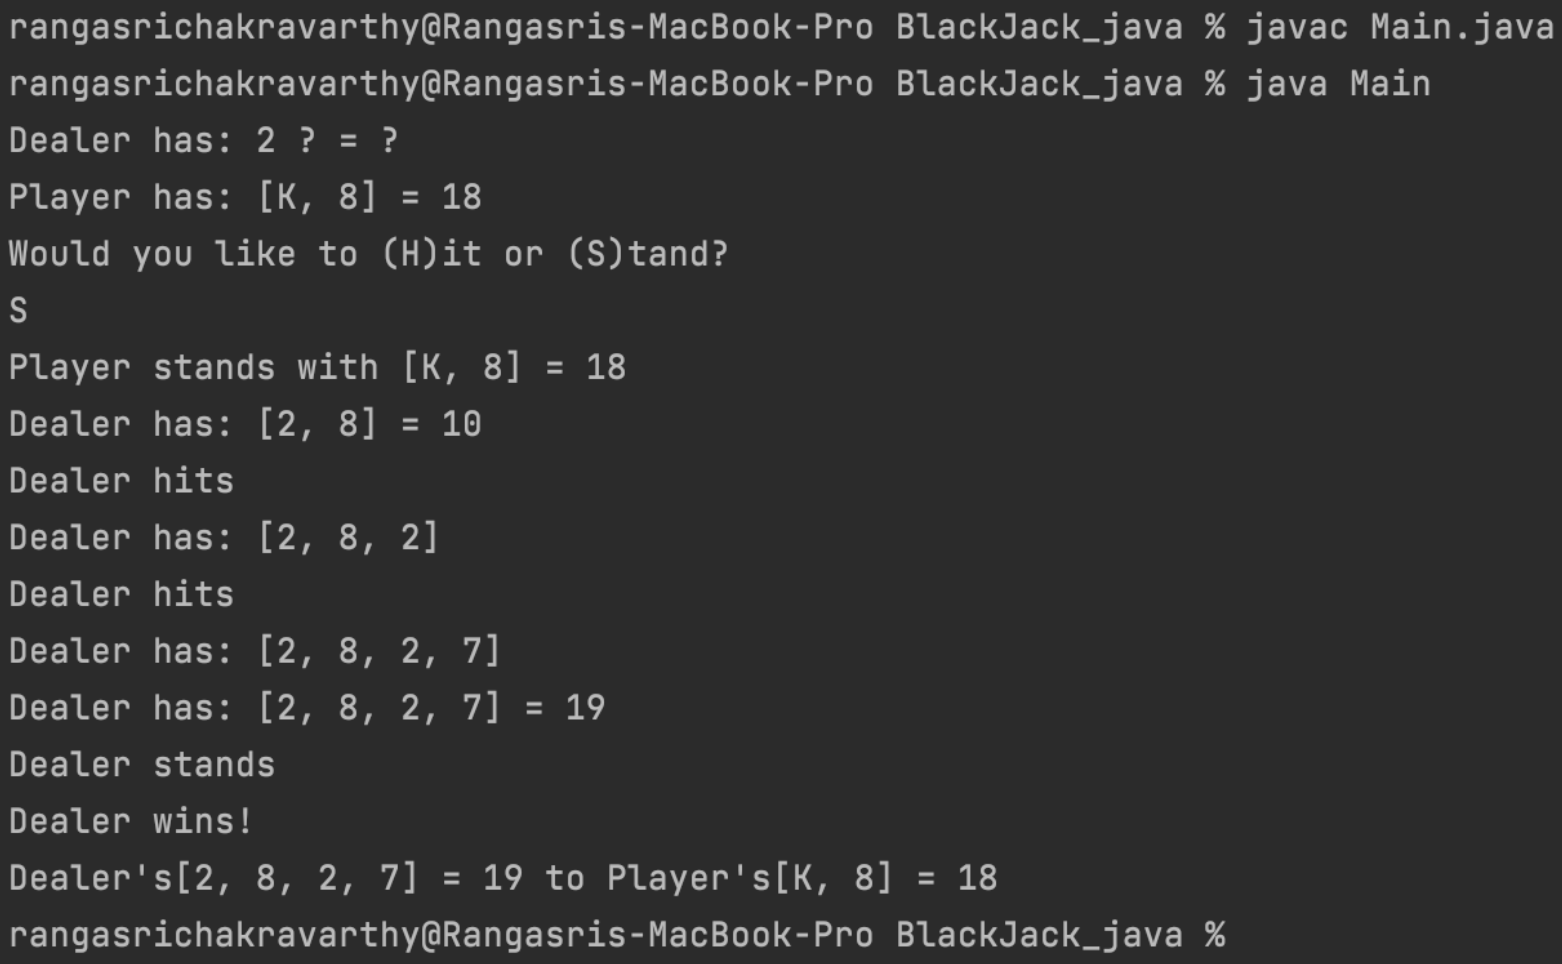
\includegraphics[height=7cm, width=15cm]{Java.png}
\caption{An example scenario of a dealer winning, that we've captured in Java}

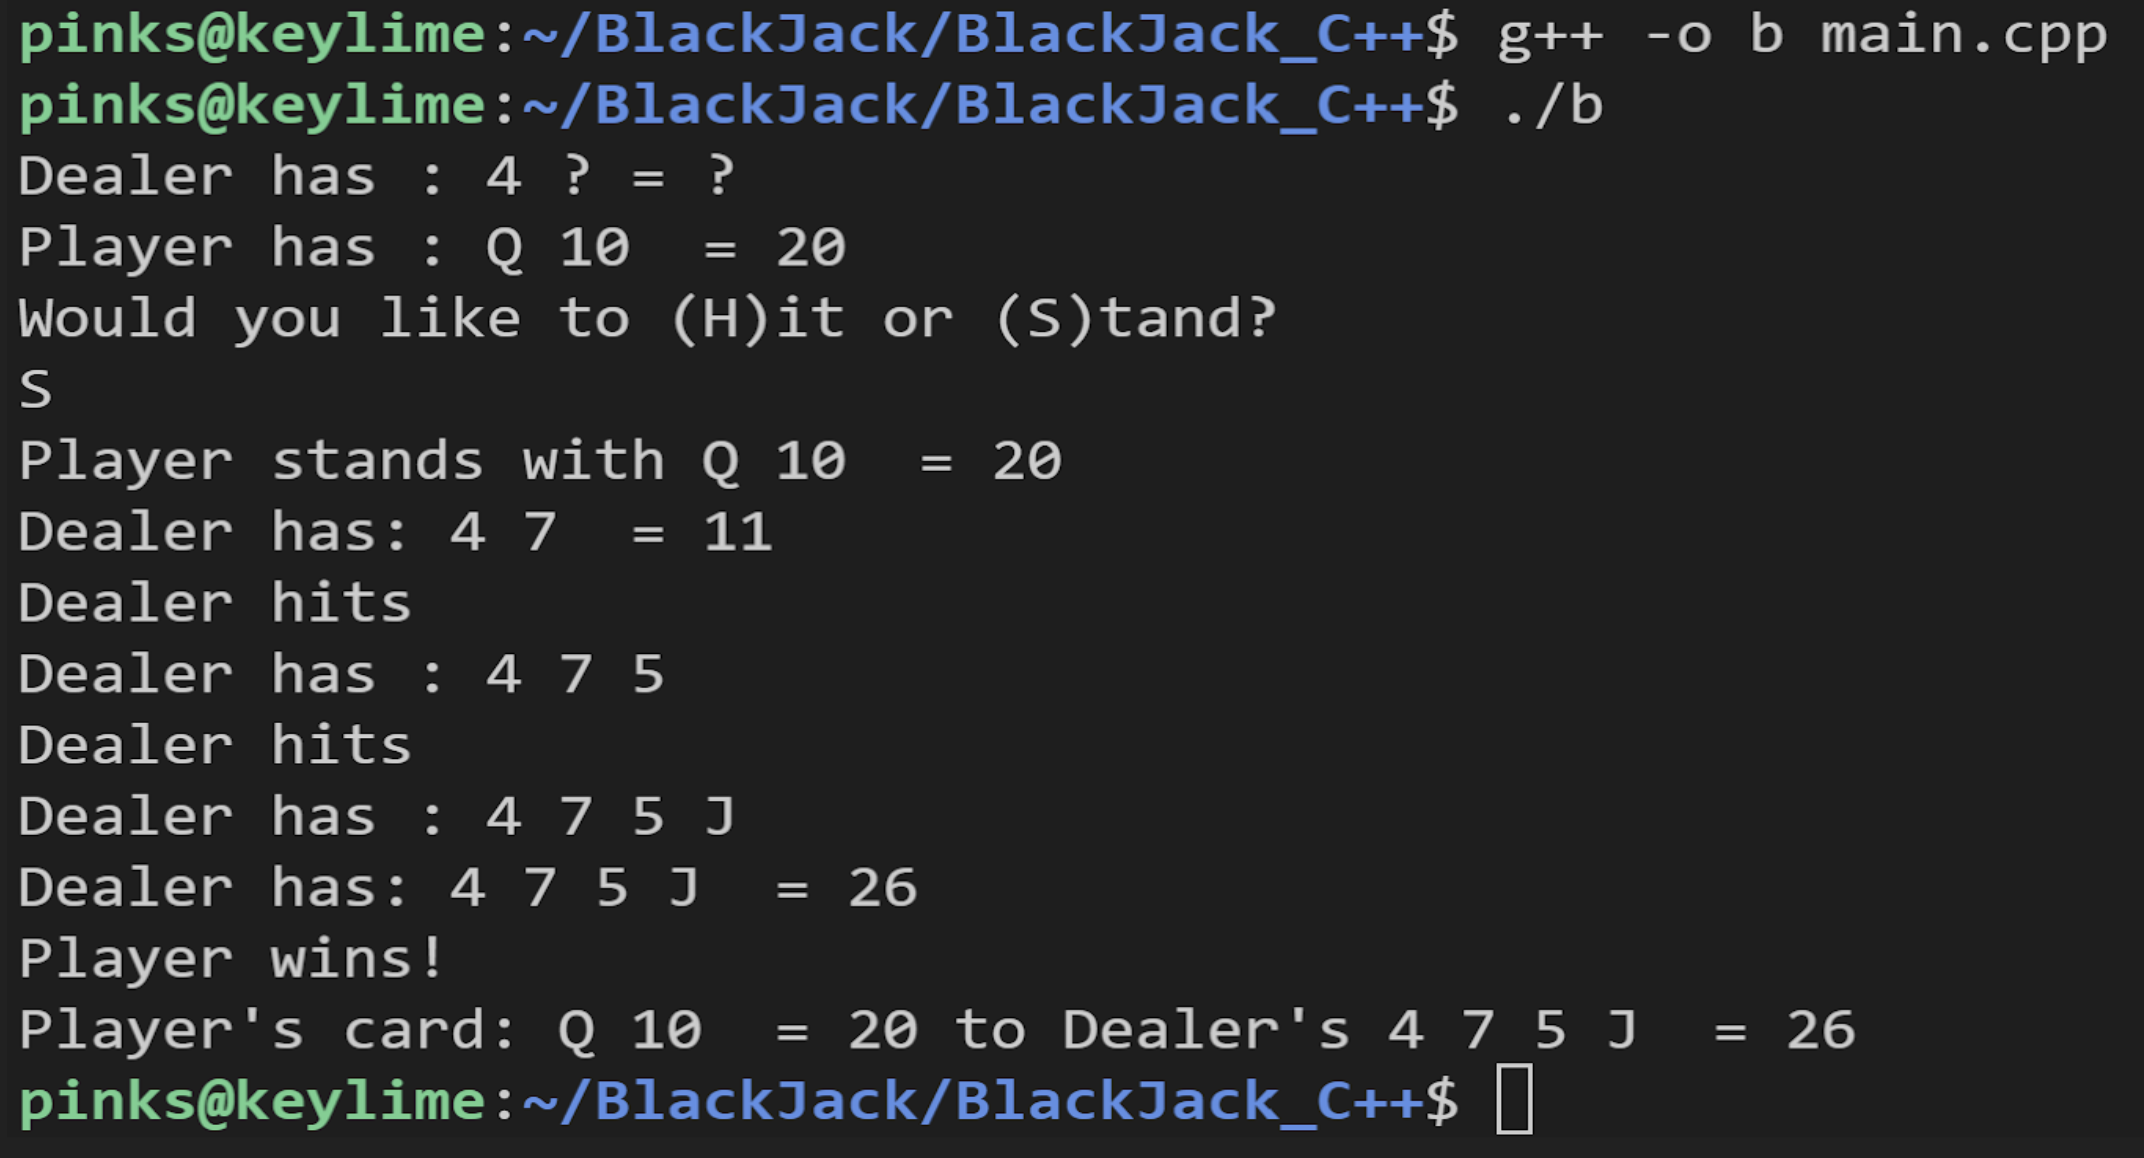
\includegraphics[height=7cm, width=15cm]{CPP.png}
\caption{An example scenario of a player winning, that we've captured in C++}
\end{figure}

\pagebreak


\section{Comparison of Programming Languages}
As a comparison based project, we've implemented BlackJack in 4 different languages:C++, Scala, Java, Python. In this section, we've compared the languages we've used, with the following metrics: Number of lines of code, Time of execution in milliseconds, Development time in hours.


\begin{figure}[h] 
\centering
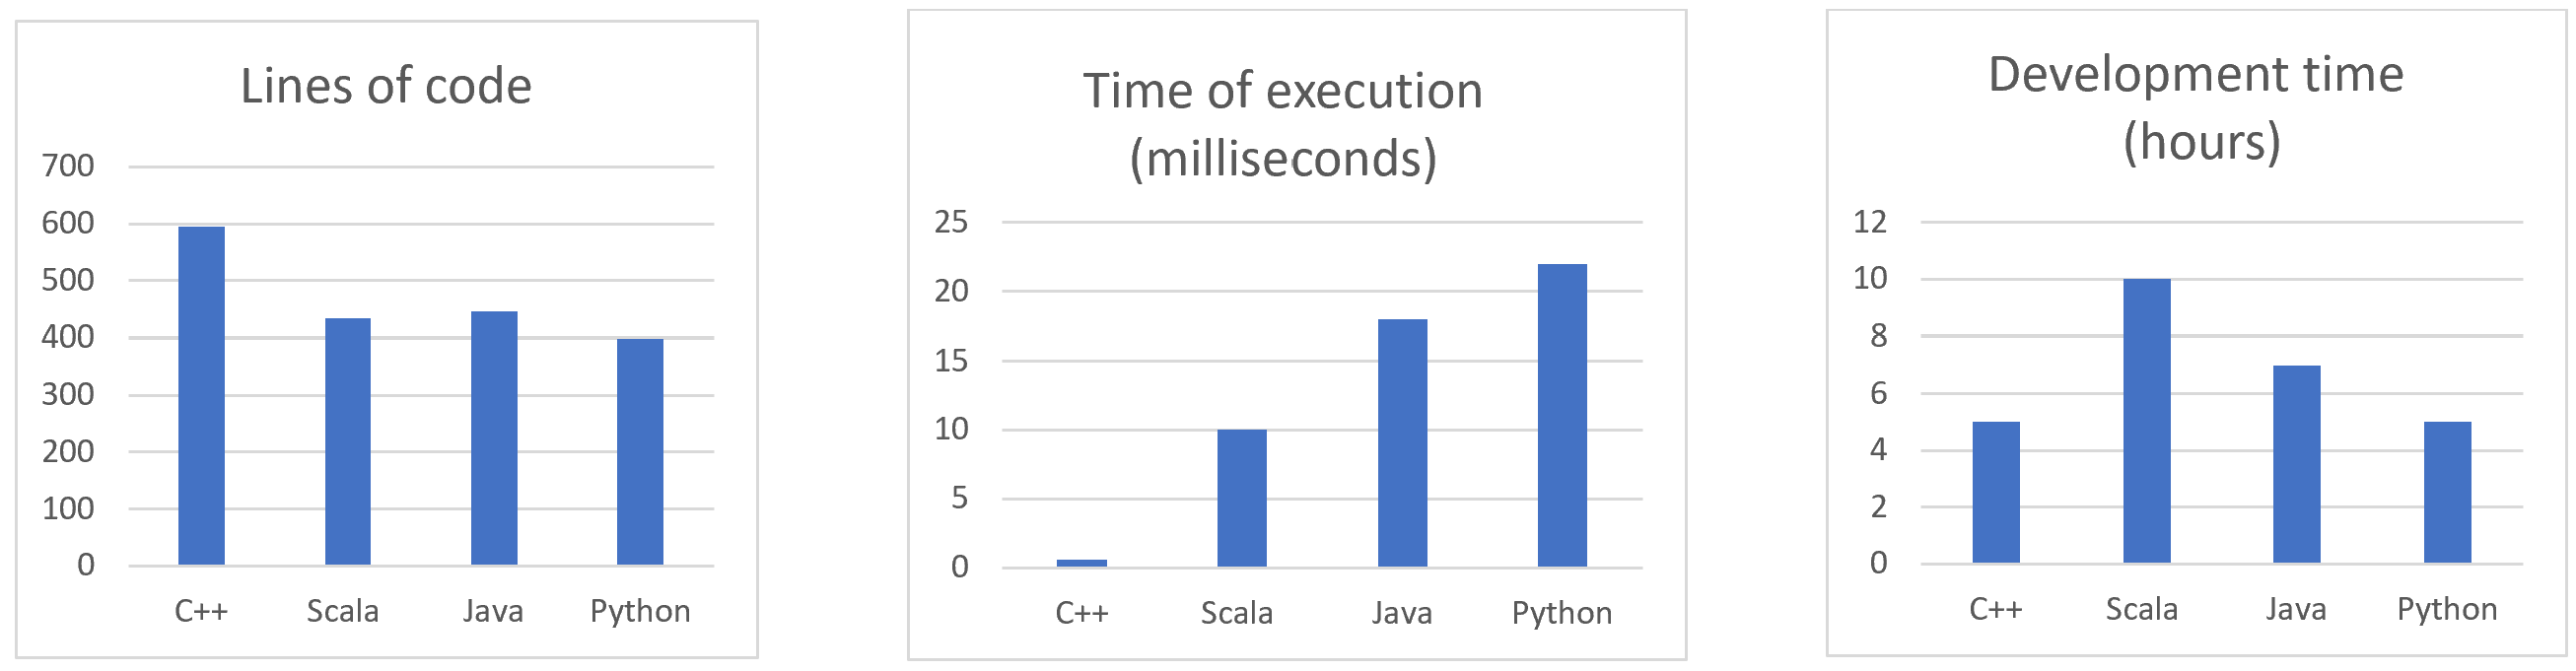
\includegraphics[height=6cm, width=18cm]{comp.png}
\caption{comparative analysis of all programming languages we've used}
\end{figure}

As we can see from the graph, it was the easiest to implement in Python because of the language's simplicity and vast library. But when it came to efficiency, C++ was the best language to use, as it took the least amount of time to run. Since Python was the first language we developed this program in, and since it was new to both of us, it took some time initially. But setting up the environment, libraries and dependencies in Scala and Java took a longer time than any other language.

\section{Challenges}

\begin{itemize}
    \item \textbf{Python:} it was a bit challenging in the beginning to decide the overall flow of the program, setting the rules, deciding the data structures to use that suited that best to implement all the functionalities we needed. Since this was a new language for us, we also had to spend some time to learn mock testing. 
    \item \textbf{Java:} there were a lot of external dependencies and jars to be installed to run the program and the test files, and the initial setup took up a lot of time.
    \item \textbf{Scala:} This was a new language for us and we invested some time learning the basics. Deciding the data structure to use (mutable/ immutable),  setting up the sbt environment, installation of jar files that were needed to run the program and tests, setting up proper folder structure were all challenging.
    \item \textbf{Testing:}We tried to analyze the performance by running the program through command line for each language. Since there can be a variety of scenarios that can occur and they are randomized every time, the runtime vastly varied and we could not consider this as a proper analysis of performance. So, in addition to implementing the proposed game, we also spent some time developing tests that can mimic exact game scenarios, and implemented that for all languages.
\end{itemize}

\section{Running our code}

\textbf{Python:} All packages we've used, comes with the standard python3 installation.

To run the main program, type "python main.py" ("python3 main.py" if python3 is not your default python interpreter) in the terminal.

To run the tests, type "python tests.py" ("python3 tests.py" if python3 is not your default python interpreter) in the terminal.

\textbf{Java:} We used IntelliJ IDE to run the program and the JUnit tests. Please install all necessary jar files needed to run the JUnit tests. 

To run the main program, type "javac Main.java" to compile, and "java Main" to run the program

We used the IDE to run the tests, but if you want to run it from the terminal, please follow the steps mentioned in this \href{https://www.lambdatest.com/blog/run-junit-from-command-line/}{link}.

\textbf{Scala:} Installation of JVM and sbt is required to run the main program and the tests.

To run the main program, type "cd /BlackJack/BlackJack\_Scala/src/main/scala/BlackJack\_Scala
scalac -classpath classes Game.scala" to compile, and "scala Game" to run the program

To run the tests, type "cd /BlackJack/BlackJack\_Scala/" and then type "sbt test" which will run all the tests.

\textbf{C++:} 

To run the main program, type "g++ -o game main.cpp" to compile and run the executable file that's created by typing "./game"

To run the tests, type "g++ -o test Testrun.cpp" to compile and run the executable file that's created by typing "./test"

\section{Conclusion}

By completing the object oriented implementation of this project, we learnt 2 new languages: Python and Scala. We also learnt to implement and run test cases using mock in Python, FreeSpec from the Scalatest library in Scala, and JUnit tests in Java. It was a fun learning experience for us. Through the implementation process and performance analysis, we can conclusively say that it was the easiest to implement this project in Python and C++ was the most efficient with regards to runtime. 

\section{References}
\begin{itemize}
  \item \href{https://junit.org/junit5/}{JUnit testing}
  \item \href{https://www.lambdatest.com/blog/run-junit-from-command-line/}{Running JUnit tests from command line}.
  \item \href{https://docs.python.org/3/library/unittest.mock.html#:~:text=mock%20is%20a%20library%20for,stubs%20throughout%20your%20test%20suite.}{Python mock library}
  \item \href{https://www.scalatest.org/at_a_glance/FreeSpec}{Scala test- FreeSpec}
  \item \href{https://docs.scala-lang.org/tour/classes.html}{Scala Tutorial}
  \item \href{https://docs.scala-lang.org/tour/classes.html}{Installing sbt}
\end{itemize}

\end{document}
